\section{Object Constraint Language (OCL)}
\label{sec:ocl}

\subsection{Overview}

\hspace{1cm} As explained in the previous section, UML is a graphical language for 
visualizing system structure and behavior. However, visual modeling with UML alone 
is insufficient for developing accurate and consistent software models, as UML 
diagrams cannot express all necessary constraints. The Object Management Group (OMG) 
developed the Object Constraint Language (OCL) to address this limitation \cite{OCL}. 
OCL is a formal assertion language with precise semantics that extends UML by 
allowing developers to specify constraints that cannot be expressed graphically. 

\begin{figure}[H]
    \begin{center}
        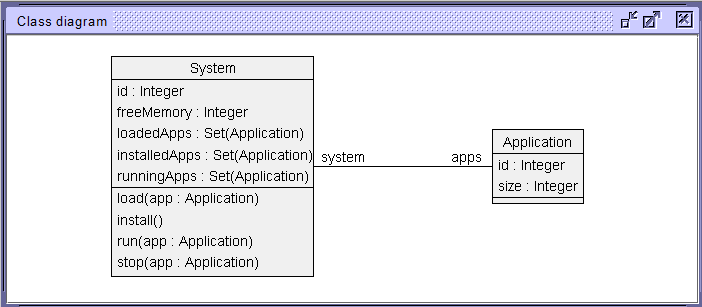
\includegraphics[width=0.8\textwidth]{figures/c1/SoftwareSystem/SS_Ver2_Gray.png}
        \caption{Class diagram of the Software System.}
        \label{fig:class_diagram_software_system}
    \end{center}
\end{figure}

To demonstrate OCL's capabilities, we'll use a simple software system model shown 
in Figure \ref{fig:class_diagram_software_system}. This model contains two classes: 
\texttt{System} and \texttt{Application}. Each class has an \texttt{id} attribute 
for unique identification. The \texttt{System} class has a \texttt{freeMemory} attribute 
representing available memory, while each \texttt{Application} has a \texttt{size} 
attribute indicating its memory requirements. The \texttt{System} class maintains three 
collections: \texttt{loadedApps}, \texttt{installedApps}, and \texttt{runningApps}, which 
track applications in different states throughout their lifecycle.

The \texttt{System} class defines the following operations:
\begin{itemize}
    \setlength{\itemsep}{0pt}
    \setlength{\parskip}{0pt}
    \setlength{\parsep}{0pt}
    \item \texttt{load(app : Application)}: downloads the application \textit{app} given as parameter and adds it to the \texttt{loadedApps} collection.
    \item \texttt{install()}: installs all the loaded applications in the \texttt{loadedApps} collection and moves them to the \texttt{installedApps} collection.
    \item \texttt{run(app : Application)}: executes the application \textit{app} given as a parameter that should be installed, adding it to the \texttt{runningApps} collection.
    \item \texttt{stop(app : Application)}: stops the application \textit{app} given as a parameter that should be running, removing it from the \texttt{runningApps} collection.
\end{itemize}


\subsection{OCL Constraints}
\hspace{1cm} Listing \ref{lst:ocl_constraints} demonstrates three typical aspects of OCL constraints. 
First, the \texttt{memoryConstraint} ensures system integrity by verifying that the 
system's free memory is non-negative, preventing memory overallocation. 
Second, the \texttt{notLoadedAndInstalled} constraint demonstrates OCL's ability to work with 
collections, ensuring that the sets of loaded and installed applications don't overlap - 
an application cannot be simultaneously in both states. This constraint uses the 
\texttt{intersection} and \texttt{isEmpty} operations to verify this condition.
Third, the \texttt{sizeConstraint} demonstrates how OCL can define 
simple rules that apply to all instances of a class, in this case ensuring all 
applications have a positive size.

\begin{lstlisting}[
    style=toclstyle, 
    caption={OCL constraints}, 
    label={lst:ocl_constraints}
]
context System
inv memoryConstraint: self.freeMemory >= 0
inv notLoadedAndInstalled: self.loadedApps->intersection(self.installedApps)->isEmpty()

context Application
inv sizeConstraint: self.size > 0
\end{lstlisting}

OCL constraints typically appear in three forms:
\begin{itemize}
    \item \textbf{Invariants:} Conditions that must always be true for all instances 
    of a class throughout their lifetime, as shown in our examples above.
    
    \item \textbf{Preconditions:} Conditions that must be true before an operation 
    executes. For instance, we could specify that an application must not be in any
    collection before the \texttt{load} operation can be performed.
    
    \item \textbf{Postconditions:} Conditions that must be true after an operation 
    completes. For example, after executing the \texttt{load} operation, the application
    must be added to the \texttt{loadedApps} collection.
\end{itemize}

Listing \ref{lst:ocl_rules} demonstrates pre- and postconditions for the \texttt{load} 
operation. The preconditions verify that (1) the application is not already in any of the
three collections (\texttt{loadedApps}, \texttt{installedApps}, or \texttt{runningApps}) 
and (2) there is enough memory available for the application. The postconditions 
ensure that (1) the application is added to the \texttt{loadedApps} collection and (2) the 
available memory is reduced by the application's size.

\begin{lstlisting}[
    style=toclstyle, 
    caption={OCL rules}, 
    label={lst:ocl_rules}
]
pre notLoaded: not self.loadedApps->includes(app) and
               not self.installedApps->includes(app) and
               not self.runningApps->includes(app)
pre enoughMemory: self.freeMemory >= app.size
post loaded: self.loadedApps = self.loadedApps@pre->including(app)
post freeMemory: self.freeMemory = self.freeMemory@pre - app.size
\end{lstlisting}

In the postcondition \texttt{freeMemory}, note the use of the \texttt{@pre} 
operator, which references the value of an attribute before the operation execution. 
This allows OCL to express constraints that relate the state before and after an 
operation. In this case, it ensures that the system's free memory after loading 
is reduced by exactly the size of the loaded application.

These examples represent just a small subset of OCL's expressive capabilities. 
OCL is type-rich, supporting basic types (Boolean, Real, Integer, String), collection 
types (Set, Bag, Sequence, OrderedSet), and special types (tuples, OclAny, OclType). 
The language provides powerful navigation capabilities for traversing relationships 
in the model, comprehensive collection operations for manipulating groups of objects, 
and quantifiers (forAll, exists) for building complex logical statements.

\subsection{OCL Limitations}

\subsubsection{Temporal Dimension}
\hspace{1cm} To illustrate the temporal limits of OCL, let us consider the following temporal 
properties of our software system: 

\begin{figure}[H]
    \begin{mdframed}
        \item \textbf{Safety 1:} An application loading must precede its run.
        \item \textbf{Safety 2:} There must be an install operation between an application's loading and its running.
        \item \textbf{Safety 3:} Each application can be loaded at most one time.
        \item \textbf{Liveness:} Every loaded application will eventually be installed.
    \end{mdframed}        
    \captionof{figure}{Temporal properties of the software system.}
    \label{fig:temporal_properties}
\end{figure}

Such temporal properties are impossible to specify in OCL without at least enriching 
the model structure with state variables. In temporal logics, we formally distinguish 
safety properties (which prevent bad events/states) from liveness properties (which 
ensure good events/states eventually happen). Safety properties consider finite 
behaviors and can sometimes be handled by modifying the model to save the system 
history, but this approach quickly becomes cumbersome and error-prone.

The fundamental limitation is that OCL expressions can only describe a single system 
state or a one-step transition from a previous state to a new state upon operation 
call. Therefore, there is no direct way to express OCL constraints involving different 
states of the model at arbitrary points in time—OCL has a very limited temporal 
dimension.

\subsubsection{Events}
\hspace{1cm} OCL also has significant limitations in handling events. An event is a predicate that 
holds at different instants of time . Mathematically, it can be represented as a 
function 
$P : \text{Time} \rightarrow {\text{true}, \text{false}}$ 
which indicates, at each instant, whether the event is triggered. The subset 
${t \in \text{Time} \mid P(t)} \subseteq \text{Time}$ 
represents all time instants at which the event $P$ occurs \cite{TOCL_Taha}.

In the object-oriented paradigm, we commonly distinguish five kinds of events: 
\begin{itemize} 
    \item \textbf{Operation call events:} Instants when a sender calls an operation of a receiver object 
    \item \textbf{Operation start events:} Instants when a receiver object starts executing an operation 
    \item \textbf{Operation end events:} Instants when the execution of an operation is finished 
    \item \textbf{Time-triggered events:} Events that occur when a specified instant is reached 
    \item \textbf{State change events:} Events that occur each time the system state changes (e.g., when the value of an attribute changes) 
\end{itemize}

OCL only provides implicit support for events through its pre- and postconditions. 
Preconditions offer an implicit universal quantification over operation call events, 
while postconditions provide an implicit universal quantification over operation end 
events. For example, a precondition on the \texttt{load} operation implicitly 
quantifies over all instances when this operation is called.

However, OCL lacks explicit constructs for the finest type of events which is state change 
events. These events, which occur when attribute values or object relationships 
change, are particularly important for dynamic systems that must detect and 
respond to changes in their operating environment. This limitation, combined with OCL's restricted temporal 
expressiveness, makes it difficult to specify many realistic system requirements 
that involve reactions to events occurring over time.
